\documentclass[a4paper,11pt]{article}
\usepackage{CJK}
\usepackage{graphicx}
\usepackage[onlyps]{altfont}
\usepackage{latexsym}
\usepackage{amsmath}
\usepackage[top=1in,bottom=1in,left=1.25in,right=1.25in]{geometry}
\usepackage[colorlinks,linkcolor=blue,anchorcolor=blue,citecolor=green]{hyperref}
\usepackage{multimedia}
\newcommand{\ud}{\mathrm{d}}
\begin{CJK}{UTF8}{gbsn}
	\author{杨梓鑫\ \ 10级物理弘毅班}
	\title{第九次计算物理作业}
	\date{学号:2010301020023}
	\begin{document}
	\maketitle
\section{Problem}
$*\mathbf{6.17.}$ None of the wave models we have considered so far include friction (i.e., damping), hence none of these waves would decay away with time. To make our simulations more realistic, add damping to the wave equation. This can be accomplished by adding a term $-2b(\partial y / \partial t)$ to the right-hand side of (6.9), corresponding to a frictional force proportional to the velocity of the string. Derive a new differencial equation that includes this term and calculate the wave pattern as a function of time. Warning: This is not a trivial calculation, but it is straight forward; for some background see Chaigne and Askenfelt (1994). You can also listen to your calculated signals if you have access to the appropriate hardware. They don't sound too bad, but they aren't quite the same as the real thing.\\\\\\

\section{Ideal Wave Whose Ends Are Fixed or Unfixed} 
I want to do this thing step by step, so we will start with ideal wave first. Following the textbook, the ideal wave obeys the wave equation
\begin{equation}
\frac{\partial ^2 y}{\partial t^2} = c^2 \frac{\partial ^2 y}{\partial x^2}
\end{equation}
which in the numerical evolution, is written as
\begin{equation}
y(i,n+1)=2[1-r^2]y(i,n)-y(i,n-1)+r^2[y(i+1,n)+y(i-1,n)],
\end{equation}
where $r \equiv c \Delta t / \Delta x$.\\\\
In Figure \ref{fig1} and Figure \ref{fig2}, the motion of the waves have been shown respectively. They both used the values $c=300$ m$/$s, $\Delta x = 10^{-3}$ m, and $r = c \Delta t / \Delta x = 1$, so that $\Delta t = 1/3 \times 10^{-5}$ s.\\
As for the initial condition, both of the figures are started with the Gaussian pluck at $x_0 = 0.2$ m as for a string length of $1$ m. And 
\begin{equation}
y_0 (x) = \mathrm{exp}[-k(x-x_0)^2].
\end{equation}
Another point worth to mention is that the two figure plotted the behaviors of two waves at exactly the same time, thus the comparison of them shows clearly the influence of the boundary condition on the solution to the differential equation, in this case, the state of the ends of the string on the propagation of the wave, resulting to the distinction of reflective wave.


\begin{figure}[htbp]
\centering
\includegraphics[trim=2.5cm 0 0 2cm]{/home/alexandra/Chap6/fixed_Ideal/WavePro5.pdf}
\caption{\sf \small Ideal wave whose ends are fixed.}
\label{fig1}
\end{figure}
\begin{figure}[htbp]
\centering
\includegraphics[trim=2.5cm 0 0 2cm]{/home/alexandra/Chap6/unfixed_Ideal/unfixedIdealWavePro.pdf}
\caption{\sf \small Ideal wave whose ends are unfixed.}
\label{fig2}
\end{figure}

\section{Frequency Spectrum}
\normalsize\qquad Recording the displacement of some point on the string between every time interval $\Delta t$, we can get the signal of 
the any wave. In Figure \ref{fig3}, the signal of our Gaussian plucked string with fixed ends has been created in this way. Then by performing the fast Fourier transformation (FFT) and plotting the sum of the modulo of the Fourier components at each frequency, as a function of the frequency, the power spectrum of the signal is obtained. Figure \ref{fig4} is created in this way, the solid curve part of it using the signal in the Figure \ref{fig3}.\\
$\qquad$ Though in the higher frequency part of the spectrum the two curve do not consent, the very first peaks of them, corresponing to the fundamental frequency, however, coincide exactly with each other, which is approximately $150$ Hz according to the data used in the plotting.\\\\ 

\begin{figure}[htbp]
\centering
\includegraphics[trim=0 1cm 0 0, scale=0.65]{/home/alexandra/Chap6/Frequency_Spec/FixedIdealStrVsT.pdf}
\caption{\sf \footnotesize Signal from a vibrating string. The string was excited with a Gaussian initial pluck at the middle of the string, and the displacement a distance 5 percent from one end was reocred. The other parameters in the simulation were the same as in Figure \ref{fig1}.}
\label{fig3}
\end{figure}

\begin{figure}[htbp]
\centering
\includegraphics[trim=0 0.3cm 0 -1cm, scale=0.8]{/home/alexandra/Chap6/Frequency_Spec/FixedIdealComb.pdf}
\caption{\sf \footnotesize The solid curve shows the power spectrum found when the string was excited at the center. And for comparison, the dotted curve is the power spectrum obtained when the string was excited 5 percent from its center.}
\label{fig4}
\end{figure}

\section{Realistic String}
\normalsize By refering to (somewhat) realistic string, our textbook only considers the stiffness of the real string, and leaving the frictional losses, aka damping, to the exercises, which is the one we will try to deal with in the next section.\\
Stiffness is added to the ideal model by an additional term in the original wave equation $(1)$,
\begin{equation}
\frac{\partial ^2 y}{\partial t^2} = c^2 \left(\frac{\partial ^2 y}{\partial x^2}-\epsilon L^2 \frac{\partial ^4 y}{\partial x^4}\right)
\end{equation}
which gives a recalculation in the numerical evolution, $(2)$ turning into
\begin{eqnarray*}
y(i,n+1)&=&[2-2r^2-6\epsilon r^2 M^2]y(i,n)-y(i,n-1)\\
&+&r^2[1+4\epsilon M^2][y(i+1,n)+y(i-1,n)]\\
&-&\epsilon r^2 M^2[y(i+2,n)+y(i-2,n)],
\end{eqnarray*}
where $M=L/\Delta x$ is the number of spatial number units along the string.Here in Figure \ref{fig5}, we employed this method to our fixed-end string and conducted the FFT to transfer to the frequency space to obtain the Power spectra for different value of stiffness $\epsilon$.\\\\\\\\

\begin{figure}[htbp]
\centering
\includegraphics[trim=0 0 0 -1cm]{/home/alexandra/Chap6/Real/RealWave.pdf}
\caption{\sf \footnotesize Power spectra for somewhat realistic strings. In all cases the strings was excited 5 percent off center, the displacement 5 percent from one end was analyzed, and we used $\Delta t = \Delta x/(4c)$ to ensure stability for all values of $\epsilon$ employed.}
\label{fig5}
\end{figure}

\newpage

\section{Piano Strings}
\normalsize Finally we are about to solve the problem in the beginning now. The additional damping term further revises the wave equation $(1)$ to
\begin{equation}
\frac{\partial ^2 y}{\partial t^2} = c^2 \left(\frac{\partial ^2 y}{\partial x^2}-\epsilon L^2 \frac{\partial ^4 y}{\partial x^4}\right)-2b\frac{\partial  y}{\partial t},
\end{equation}
which leads to $(2)$ turning into
\begin{eqnarray*}
y\left(i,n+1\right)&=&\left[2-2r^2-6\epsilon r^2 M^2-2b\Delta t\right]y\left(i,n\right)-\left(1-2b\Delta t\right)y\left(i,n-1\right)\\
&+&r^2\left[1+4\epsilon M^2\right]\left[y\left(i+1,n\right)+y\left(i-1,n\right)\right]\\
&-&\epsilon r^2 M^2\left[y\left(i+2,n\right)+y\left(i-2,n\right)\right].\\
\end{eqnarray*}
Perform parameters on TABLE 6.1, we find the wave signals of all three notes, $C2$, $C4$, and $C7$ in Figure \ref{fig6}.\\\\

\begin{figure}[htbp]
\centering
\includegraphics[trim=0 0 0 -1cm, scale=0.9]{/home/alexandra/Chap6/Piano/PianoC2Wave.pdf}
\includegraphics[trim=0 0 0 -1cm, scale=0.9]{/home/alexandra/Chap6/Piano/PianoC4Wave.pdf}
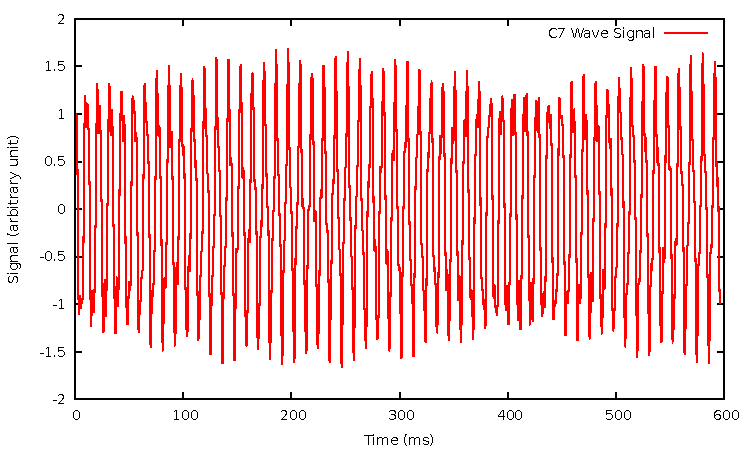
\includegraphics[trim=0 0 0 -1cm, scale=0.9]{/home/alexandra/Chap6/Piano/PianoC7Wave.pdf}
\caption{\sf \footnotesize Wave Signals for $C2$, $C4$, and $C7$.}
\label{fig6}
\end{figure}
\normalsize\noindent Click on the boxes to listen to the simulated notes and real standard notes.\\\\
\fbox{\sound[inlinesound,bitspersample=8,channels=2,automute,encoding=muLaw,samplingrate=44100]{Real life C2 note}{/home/alexandra/Note2.wav}}\qquad\qquad\qquad \qquad
\fbox{\sound[inlinesound,bitspersample=8,channels=2,automute,encoding=muLaw,samplingrate=44100]{Real life C4 note}{/home/alexandra/Note4.wav}}\qquad\qquad\qquad \qquad
\fbox{\sound[inlinesound,bitspersample=8,channels=2,automute,encoding=muLaw,samplingrate=44100]{Real life C7 note}{/home/alexandra/Note7.wav}} \\\\
\noindent
\fbox{\sound[inlinesound,bitspersample=8,channels=2,automute,encoding=muLaw,samplingrate=44100]{Calculation Result of C2 note}{/home/alexandra/PianoC2.wav}}\qquad 
\fbox{\sound[inlinesound,bitspersample=8,channels=2,automute,encoding=muLaw,samplingrate=44100]{Calculation Result of C4 note}{/home/alexandra/PianoC4.wav}}\qquad 
\fbox{\sound[inlinesound,bitspersample=8,channels=2,automute,encoding=muLaw,samplingrate=44100]{Calculation Result of C7 note}{/home/alexandra/PianoC7.wav}} \\


\end{CJK}
\end{document}
